\documentclass[11pt]{article}

\usepackage[T2A]{fontenc}
\usepackage[utf8]{inputenc}
\usepackage[russian]{babel}
\usepackage{hyperref}
\usepackage{xcolor}
 % Цвета для гиперссылок
\definecolor{linkcolor}{HTML}{0000FF} % цвет ссылок
\definecolor{urlcolor}{HTML}{FF0000} % цвет гиперссылок
 
\hypersetup{pdfstartview=FitH,  linkcolor=linkcolor,urlcolor=urlcolor, colorlinks=true}
\usepackage{hyphenat}
\hyphenation{ма-те-ма-ти-ка вос-ста-нав-ли-вать}

\usepackage[a4paper,margin=2cm]{geometry}

\usepackage{graphicx}
\usepackage{subcaption}
\usepackage{tikz}
\usepackage[intlimits]{amsmath}
\usepackage{amssymb}
\usepackage{amsmath}
\usepackage{subcaption}
\usepackage{wrapfig}
\usepackage{float}
\usepackage{fancyhdr}
\usepackage{mathtools}
\usepackage{tensor}
\usepackage{pgf}
\usepackage{array}
\usepackage[utf8]{inputenc}\DeclareUnicodeCharacter{2212}{-}


\author{Смирнов Иван }
\date{\today}
\title{Распределение коэффициента давлений крыла Onera M6}

\begin{document}
\maketitle
\begin{figure}[h!]
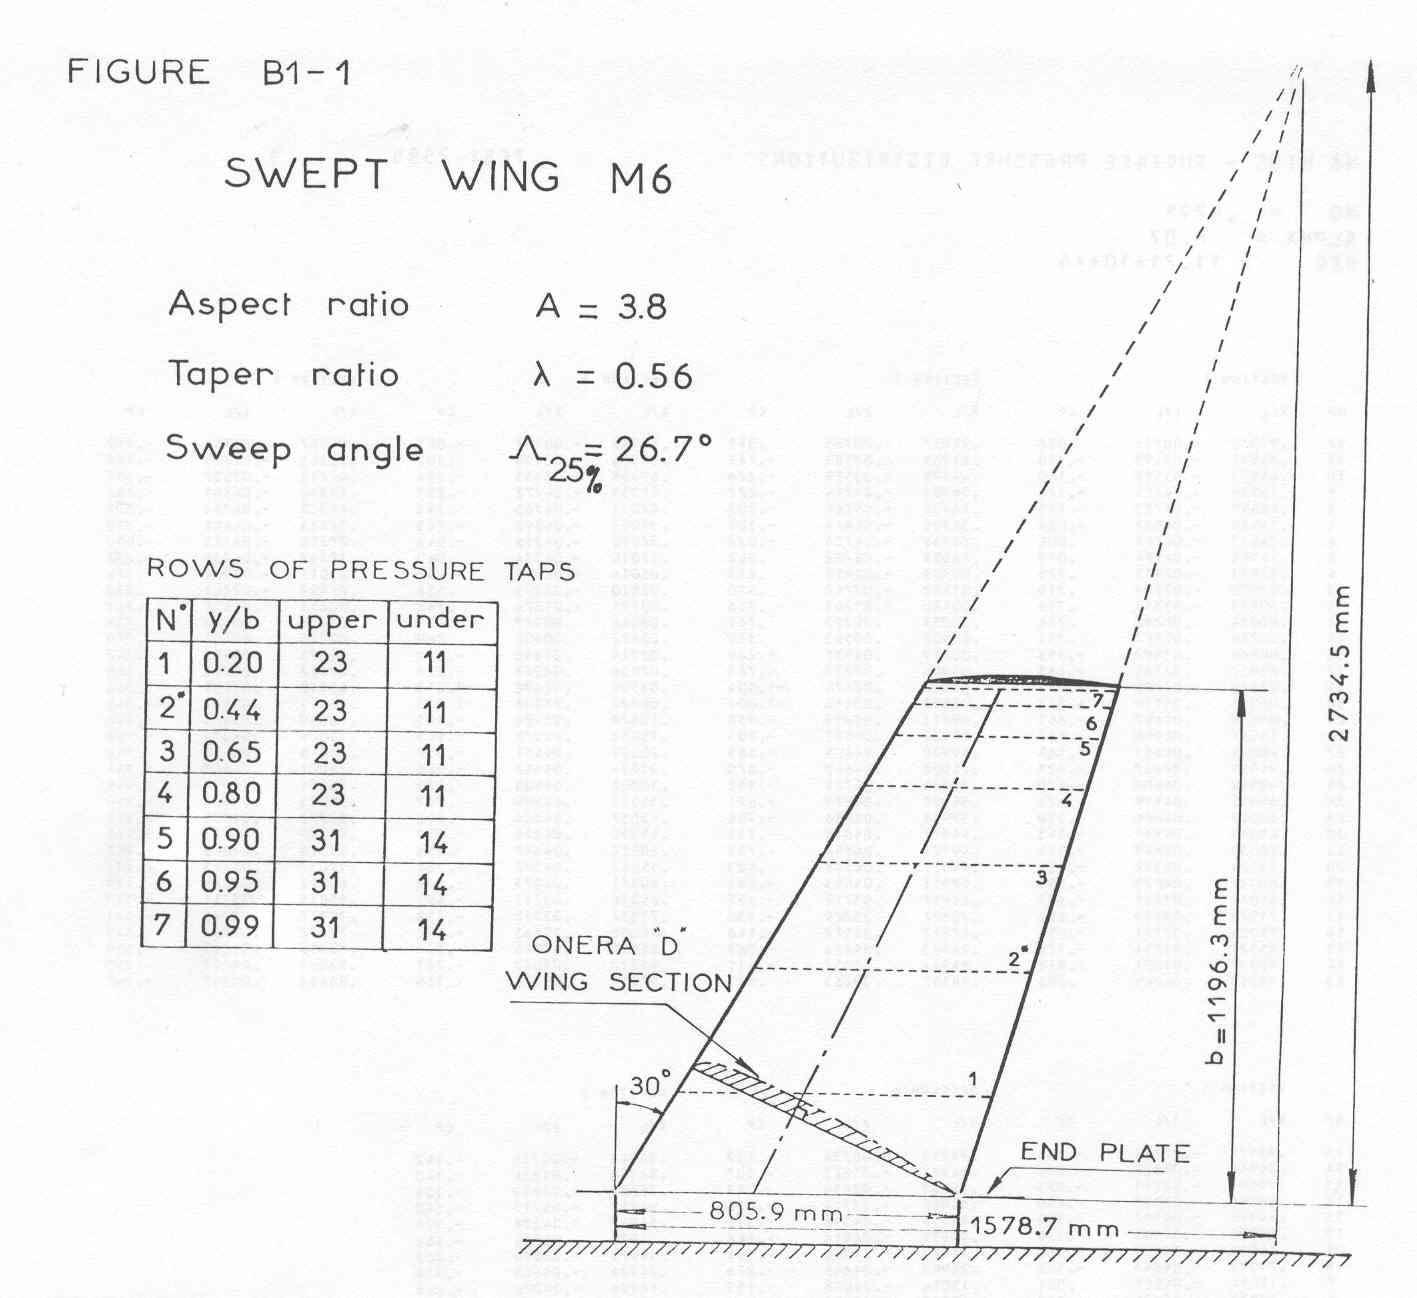
\includegraphics[width = \textwidth]{onera.jpg}
\caption{$y/b$ - отношение расстояния от начала крыла к его длине, графики ниже иллюстрируют экспериментальные и численные данные в этих местах}
\end{figure}
\noindent Давление снизу крыла выше, чем сверху - условие возникговения подъёмной силы. Также видно, что чем ближе к концу крыла, тем меньше совпадают данные, полученные численным методом, с экспериментальными данными. Возможно это связано с трудностями учёта всех условий на границах(там однозначно возникают завихрения, которые сложно описать какой-то моделью).
\newpage
    

\section*{Графики распределения коэффициента давления}
\begin{figure}[h!]
\begin{minipage}{.49\textwidth}
    \centering
    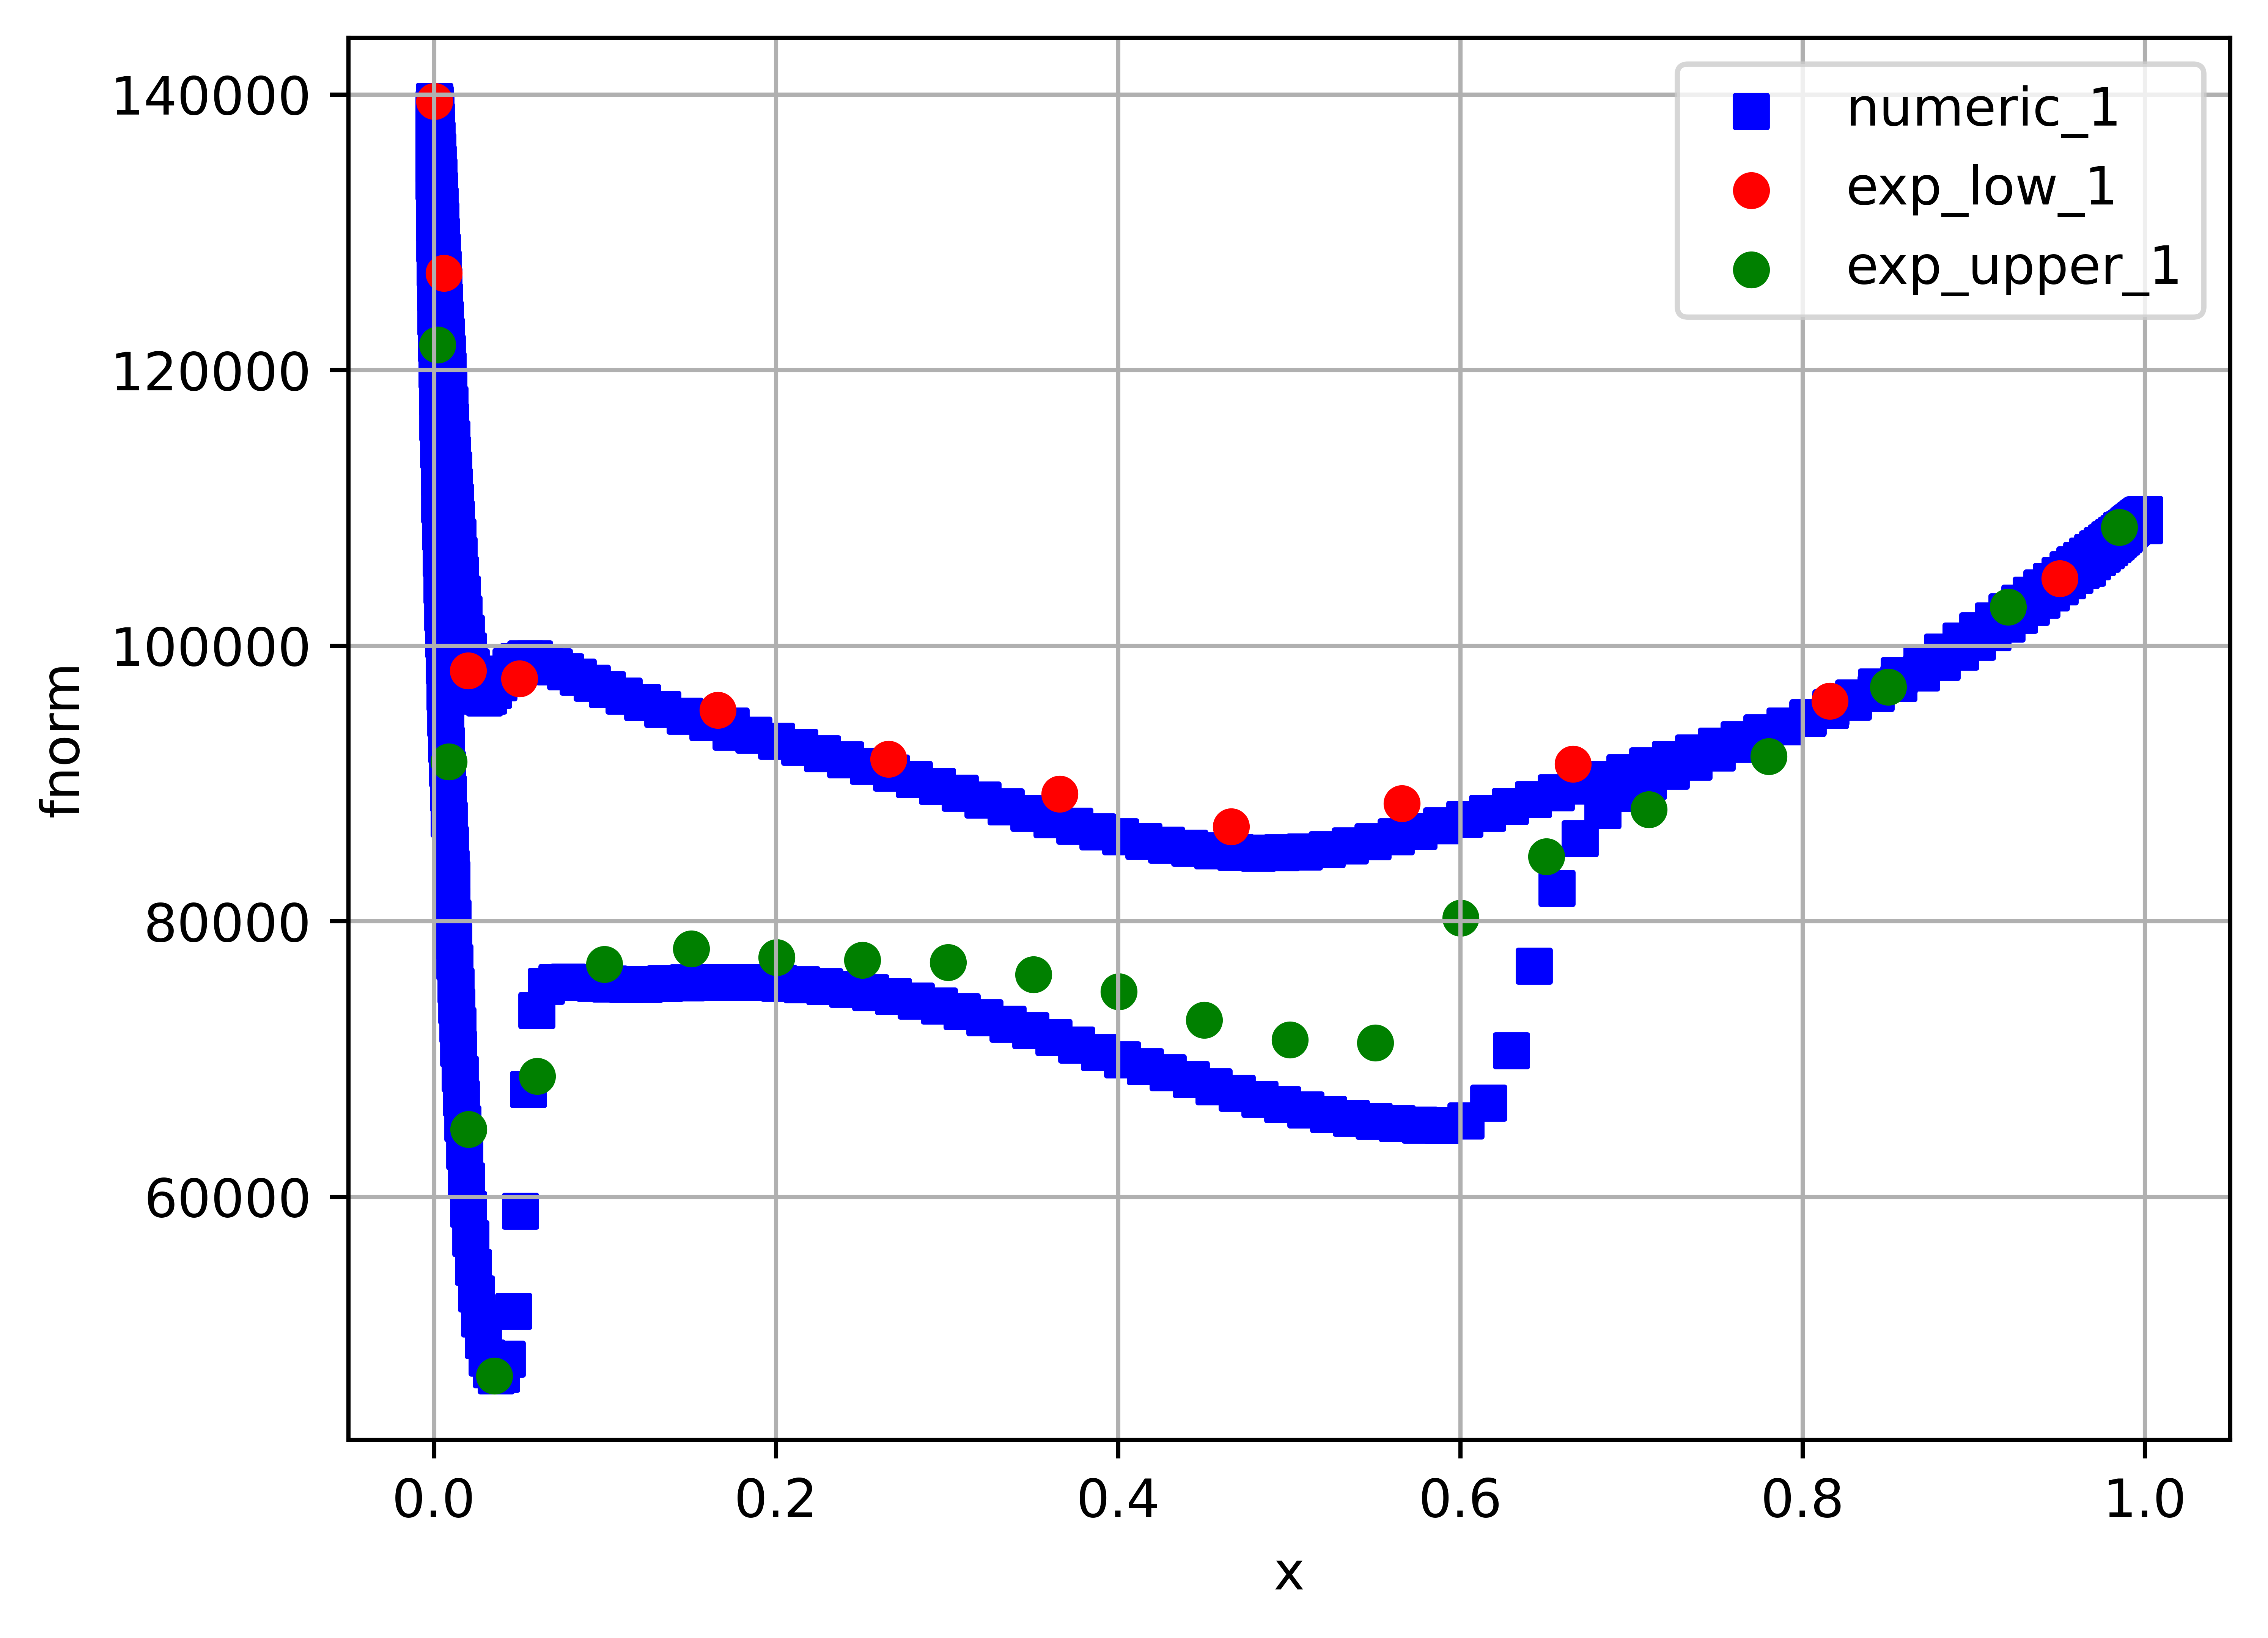
\includegraphics[width = 1\textwidth]{1.png}
\end{minipage}
\begin{minipage}{.49\textwidth}
    \centering
    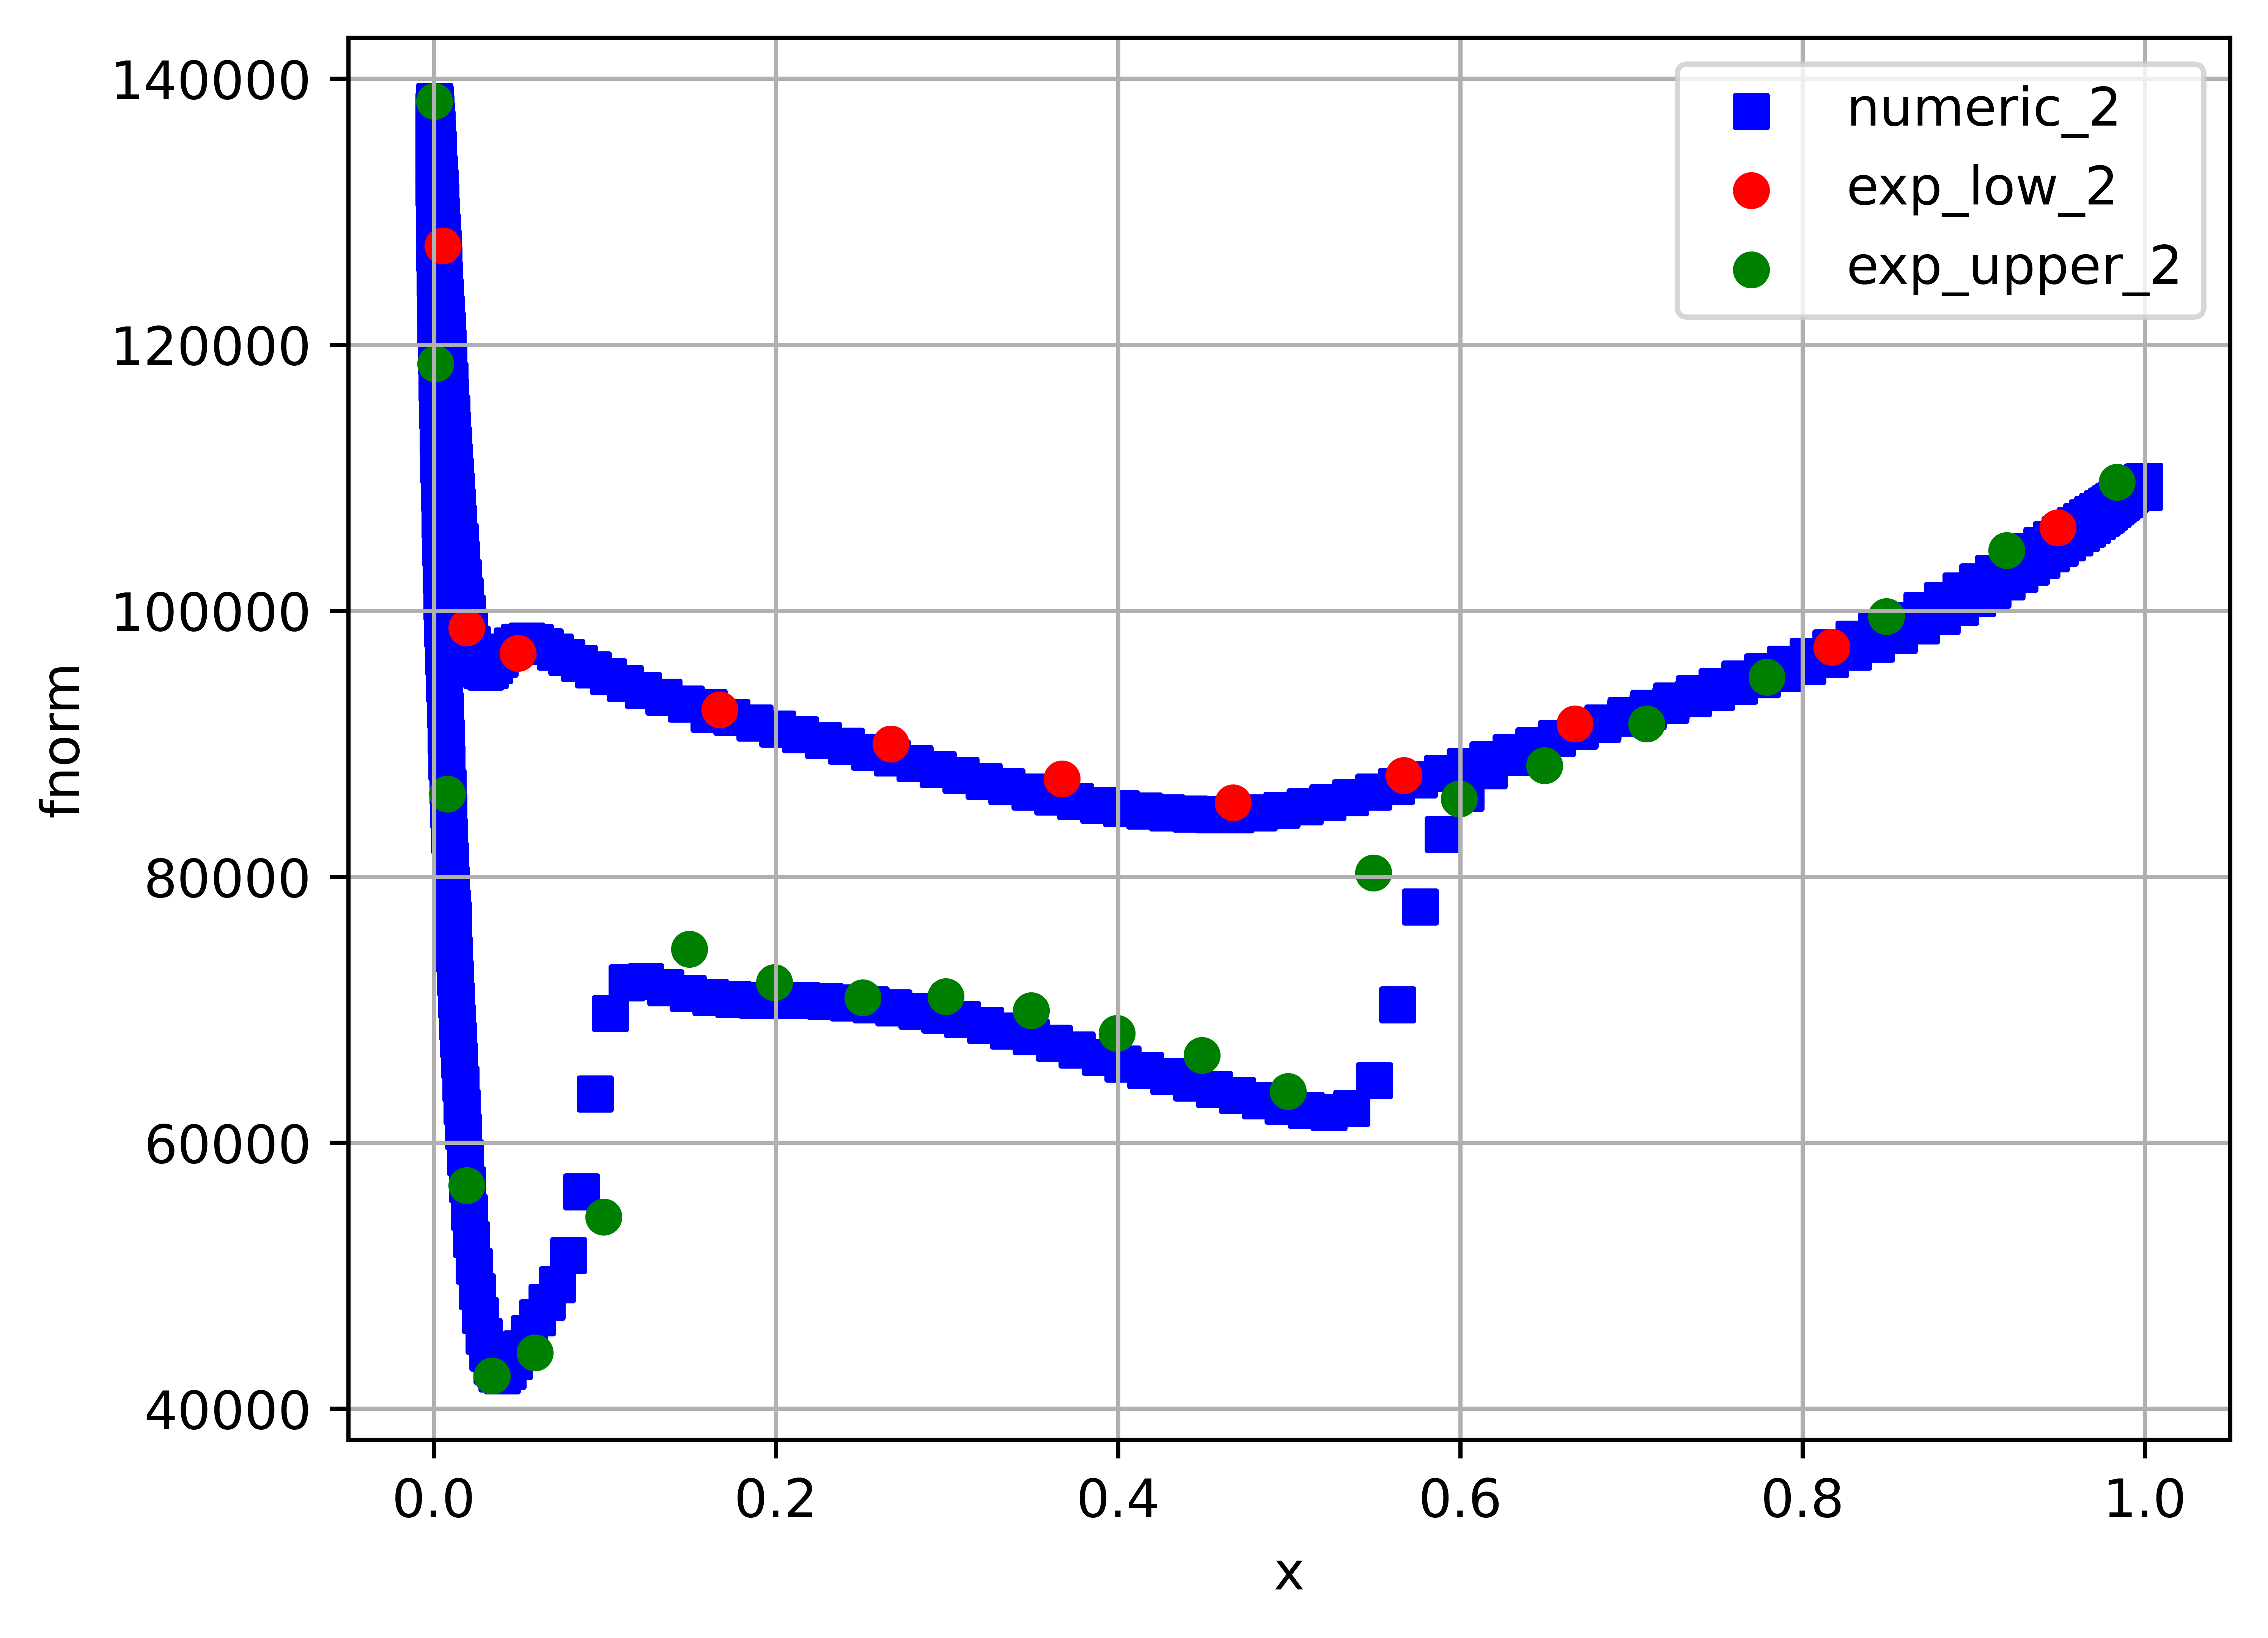
\includegraphics[width = 1\textwidth]{2.png}
\end{minipage}
\begin{minipage}{.49\textwidth}
    \centering
    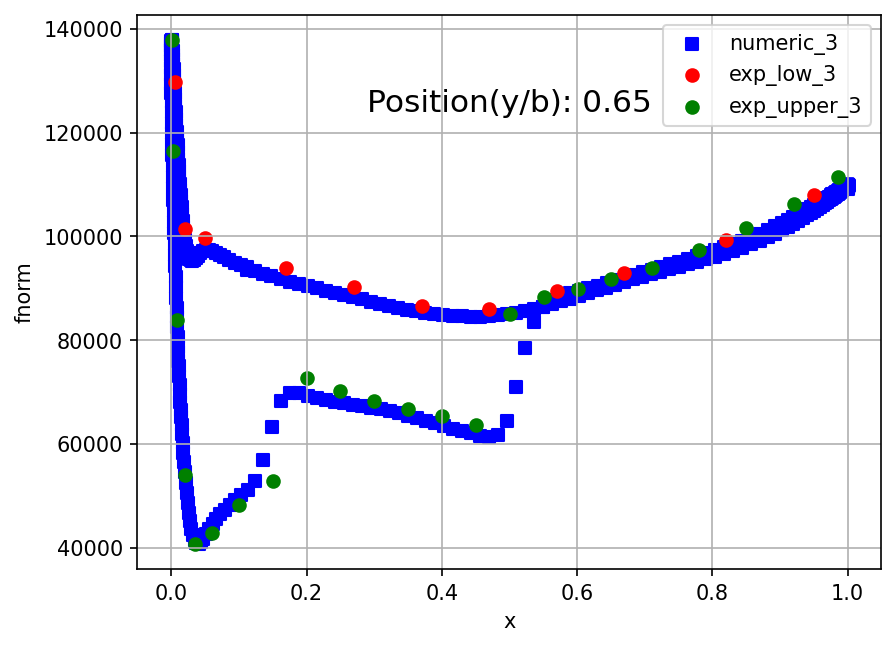
\includegraphics[width = 1\textwidth]{3.png}
\end{minipage}
\begin{minipage}{.49\textwidth}
    \centering
    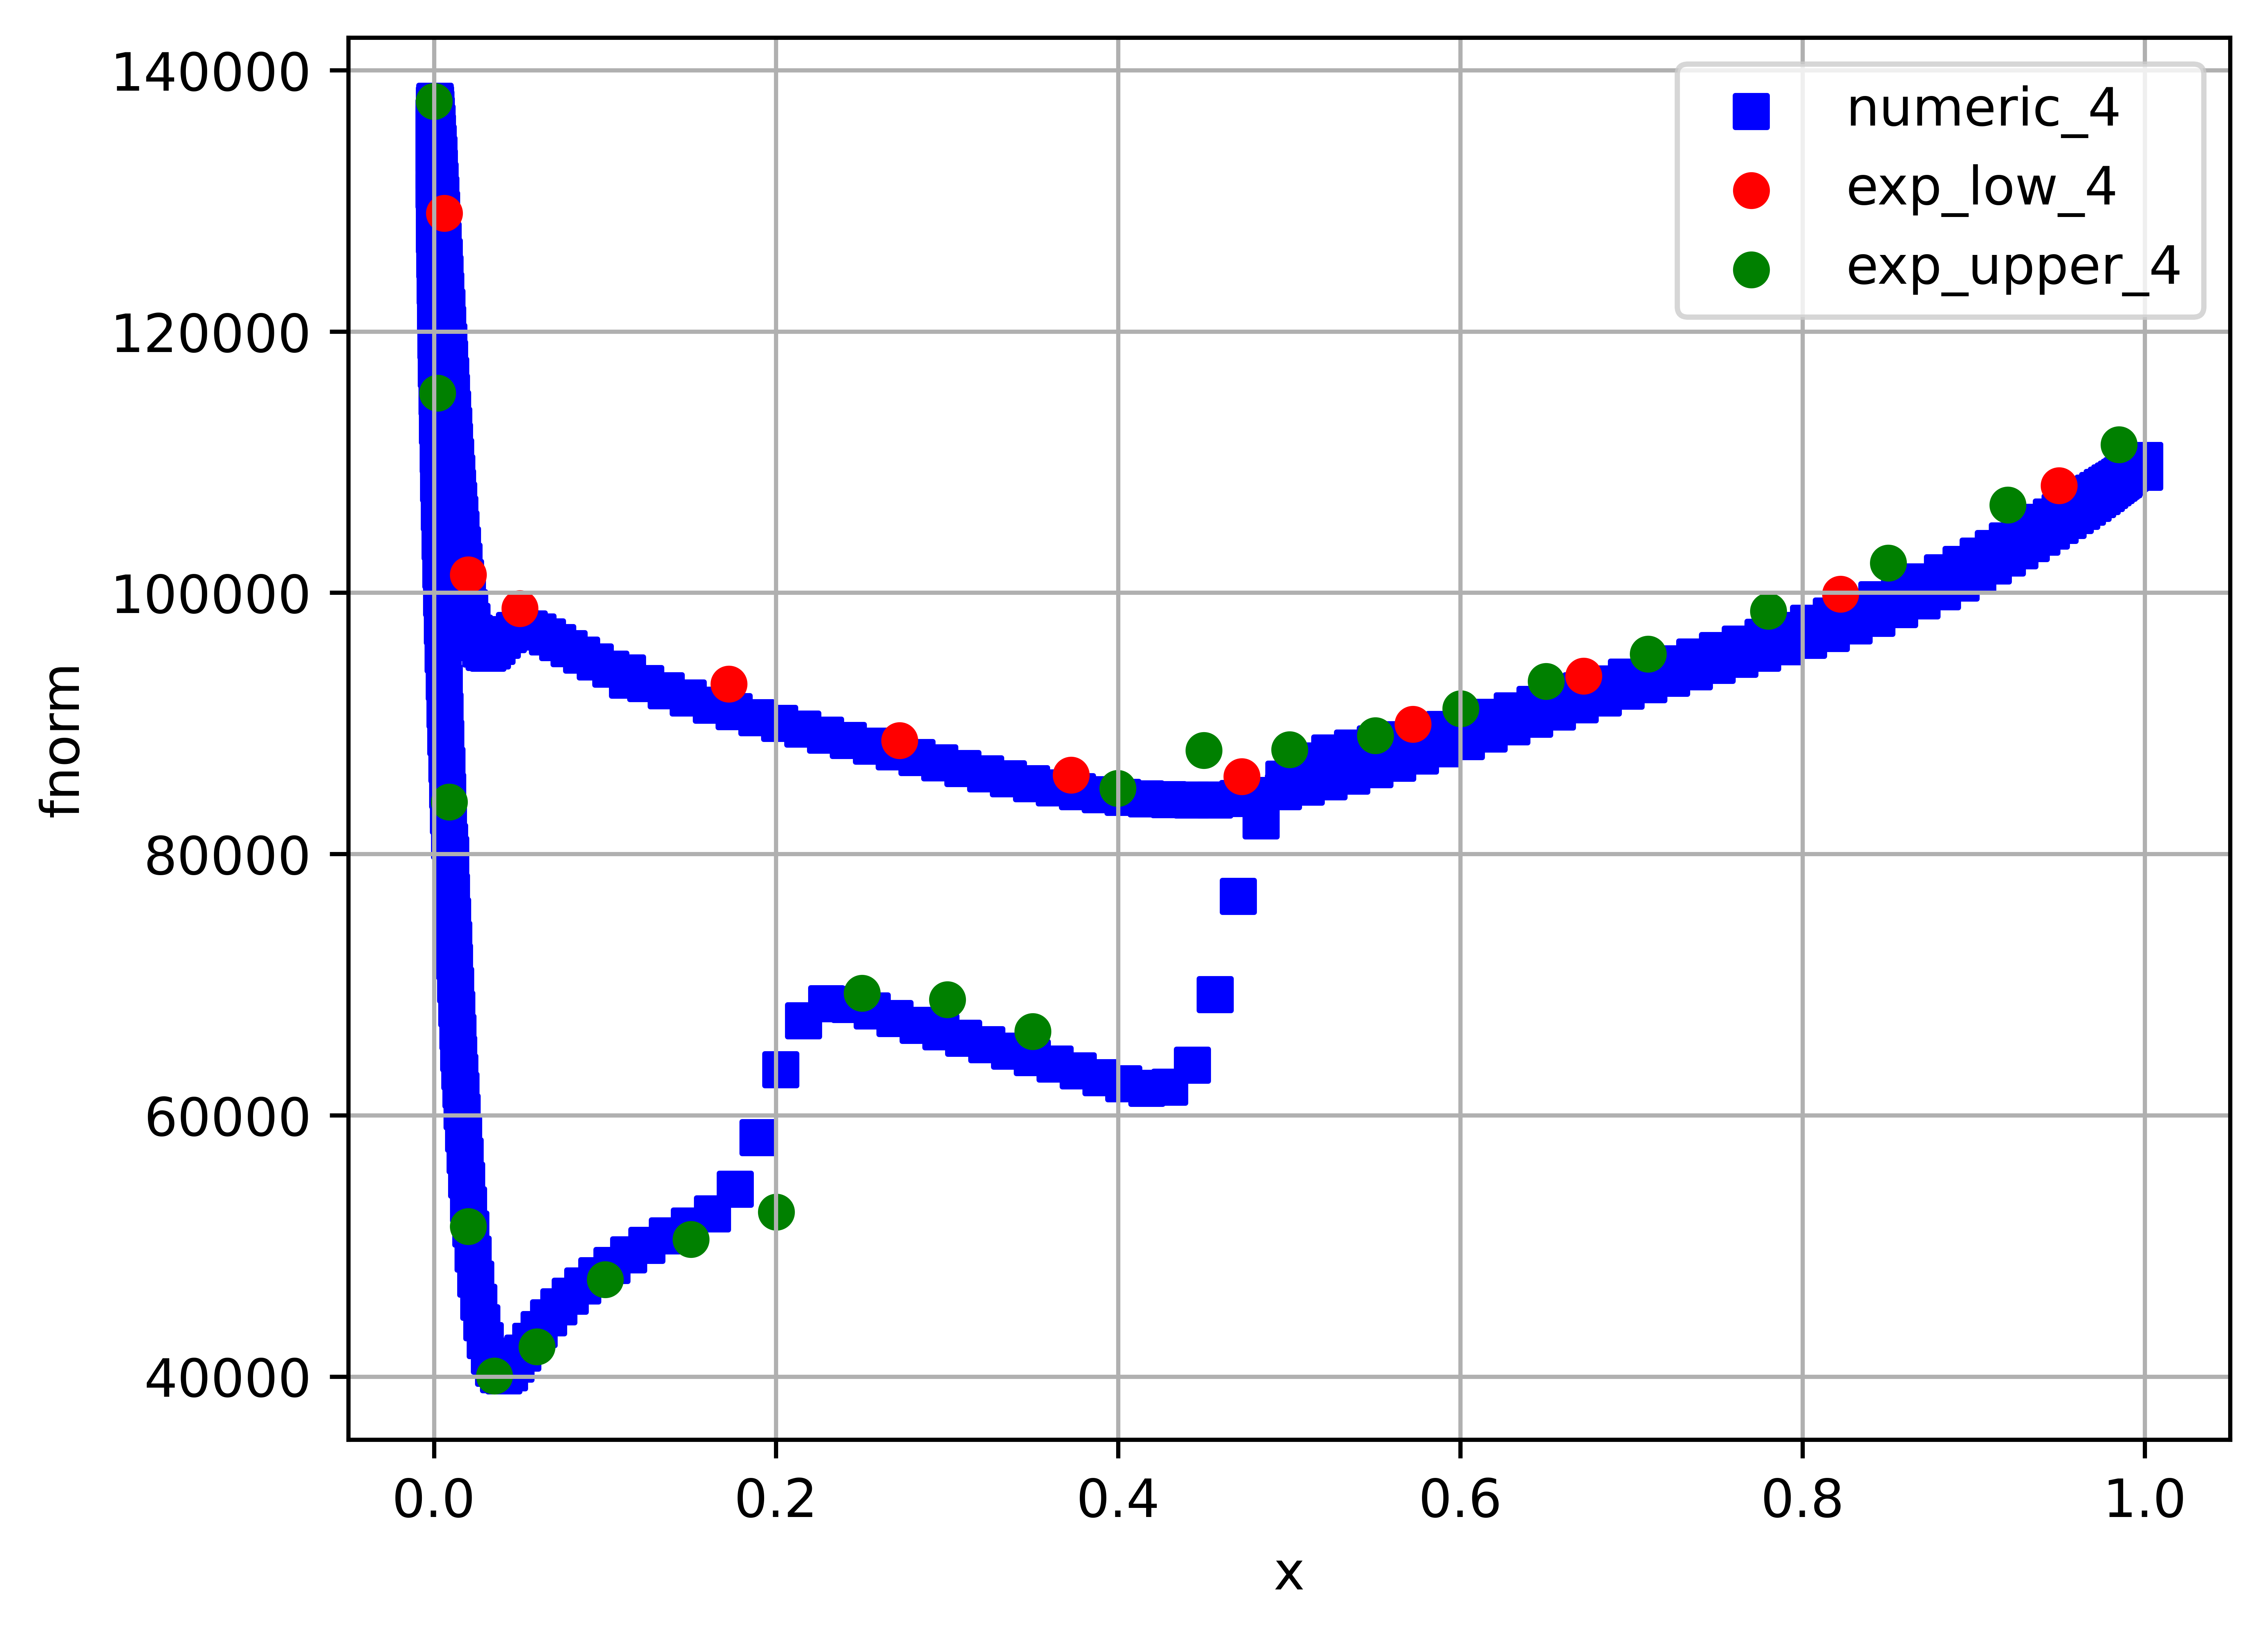
\includegraphics[width = 1\textwidth]{4.png}
\end{minipage}
\begin{minipage}{.49\textwidth}
    \centering
    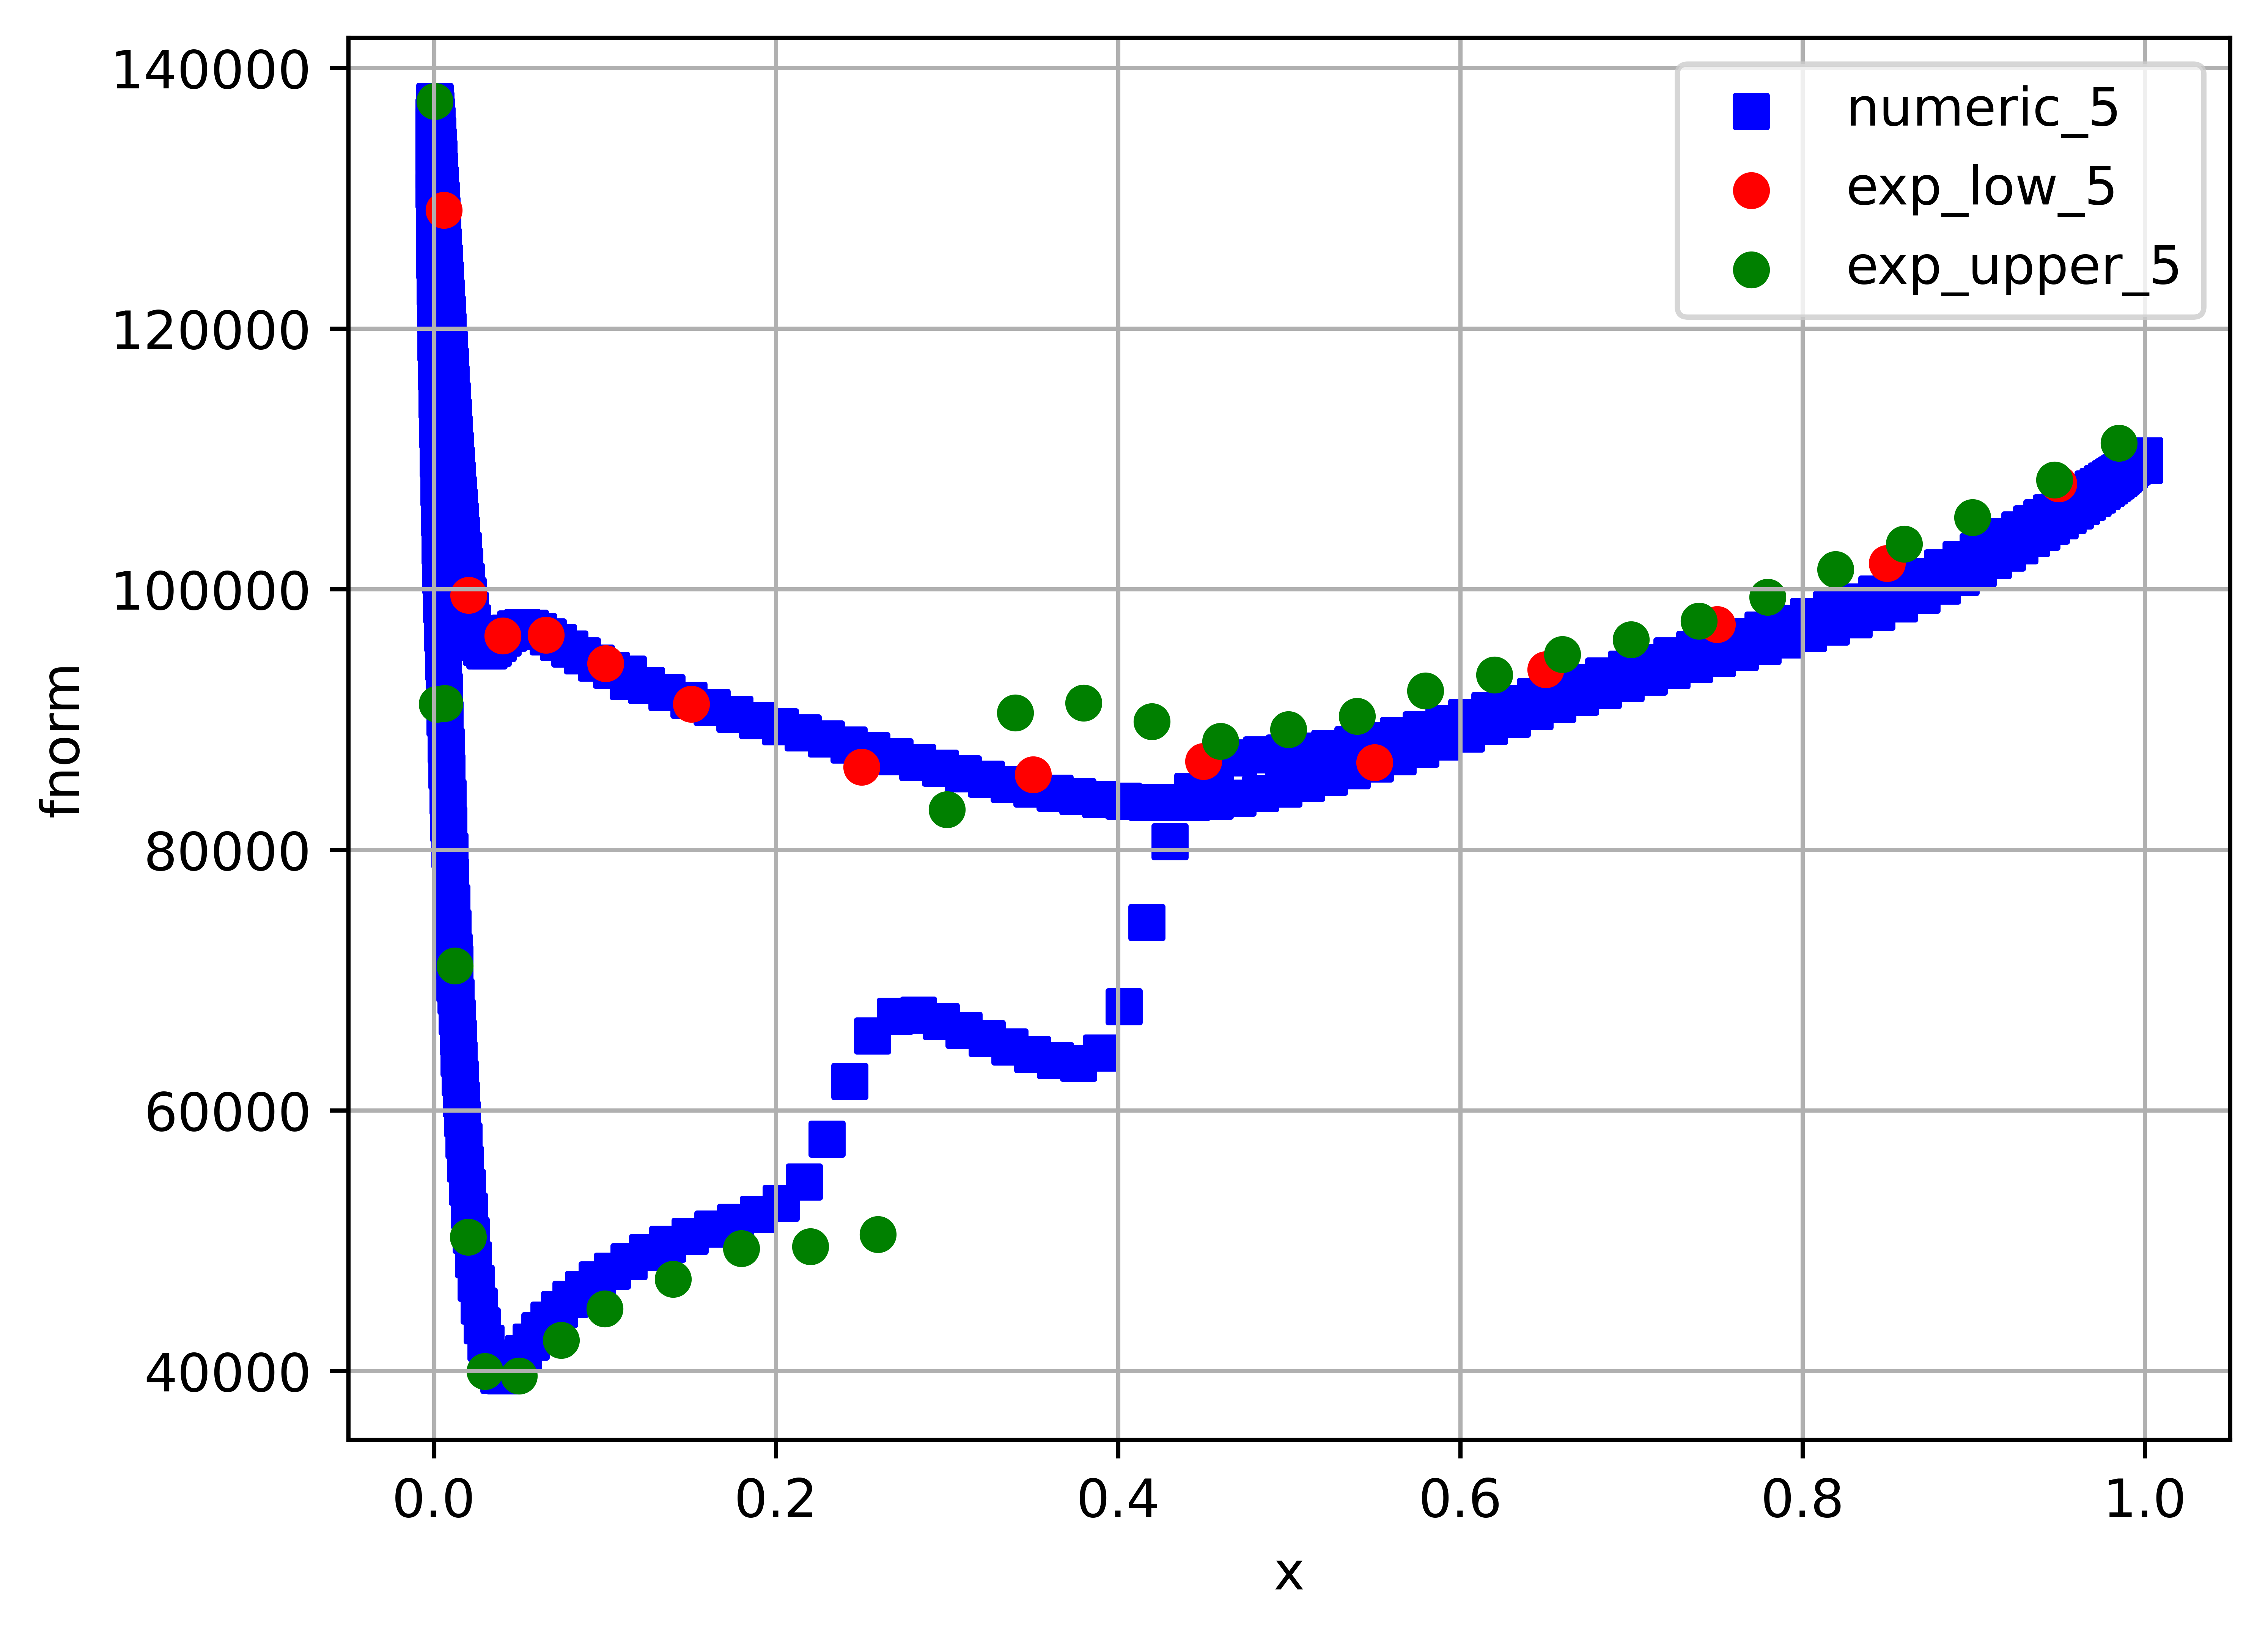
\includegraphics[width = 1\textwidth]{5.png}
\end{minipage}
\begin{minipage}{.49\textwidth}
    \centering
    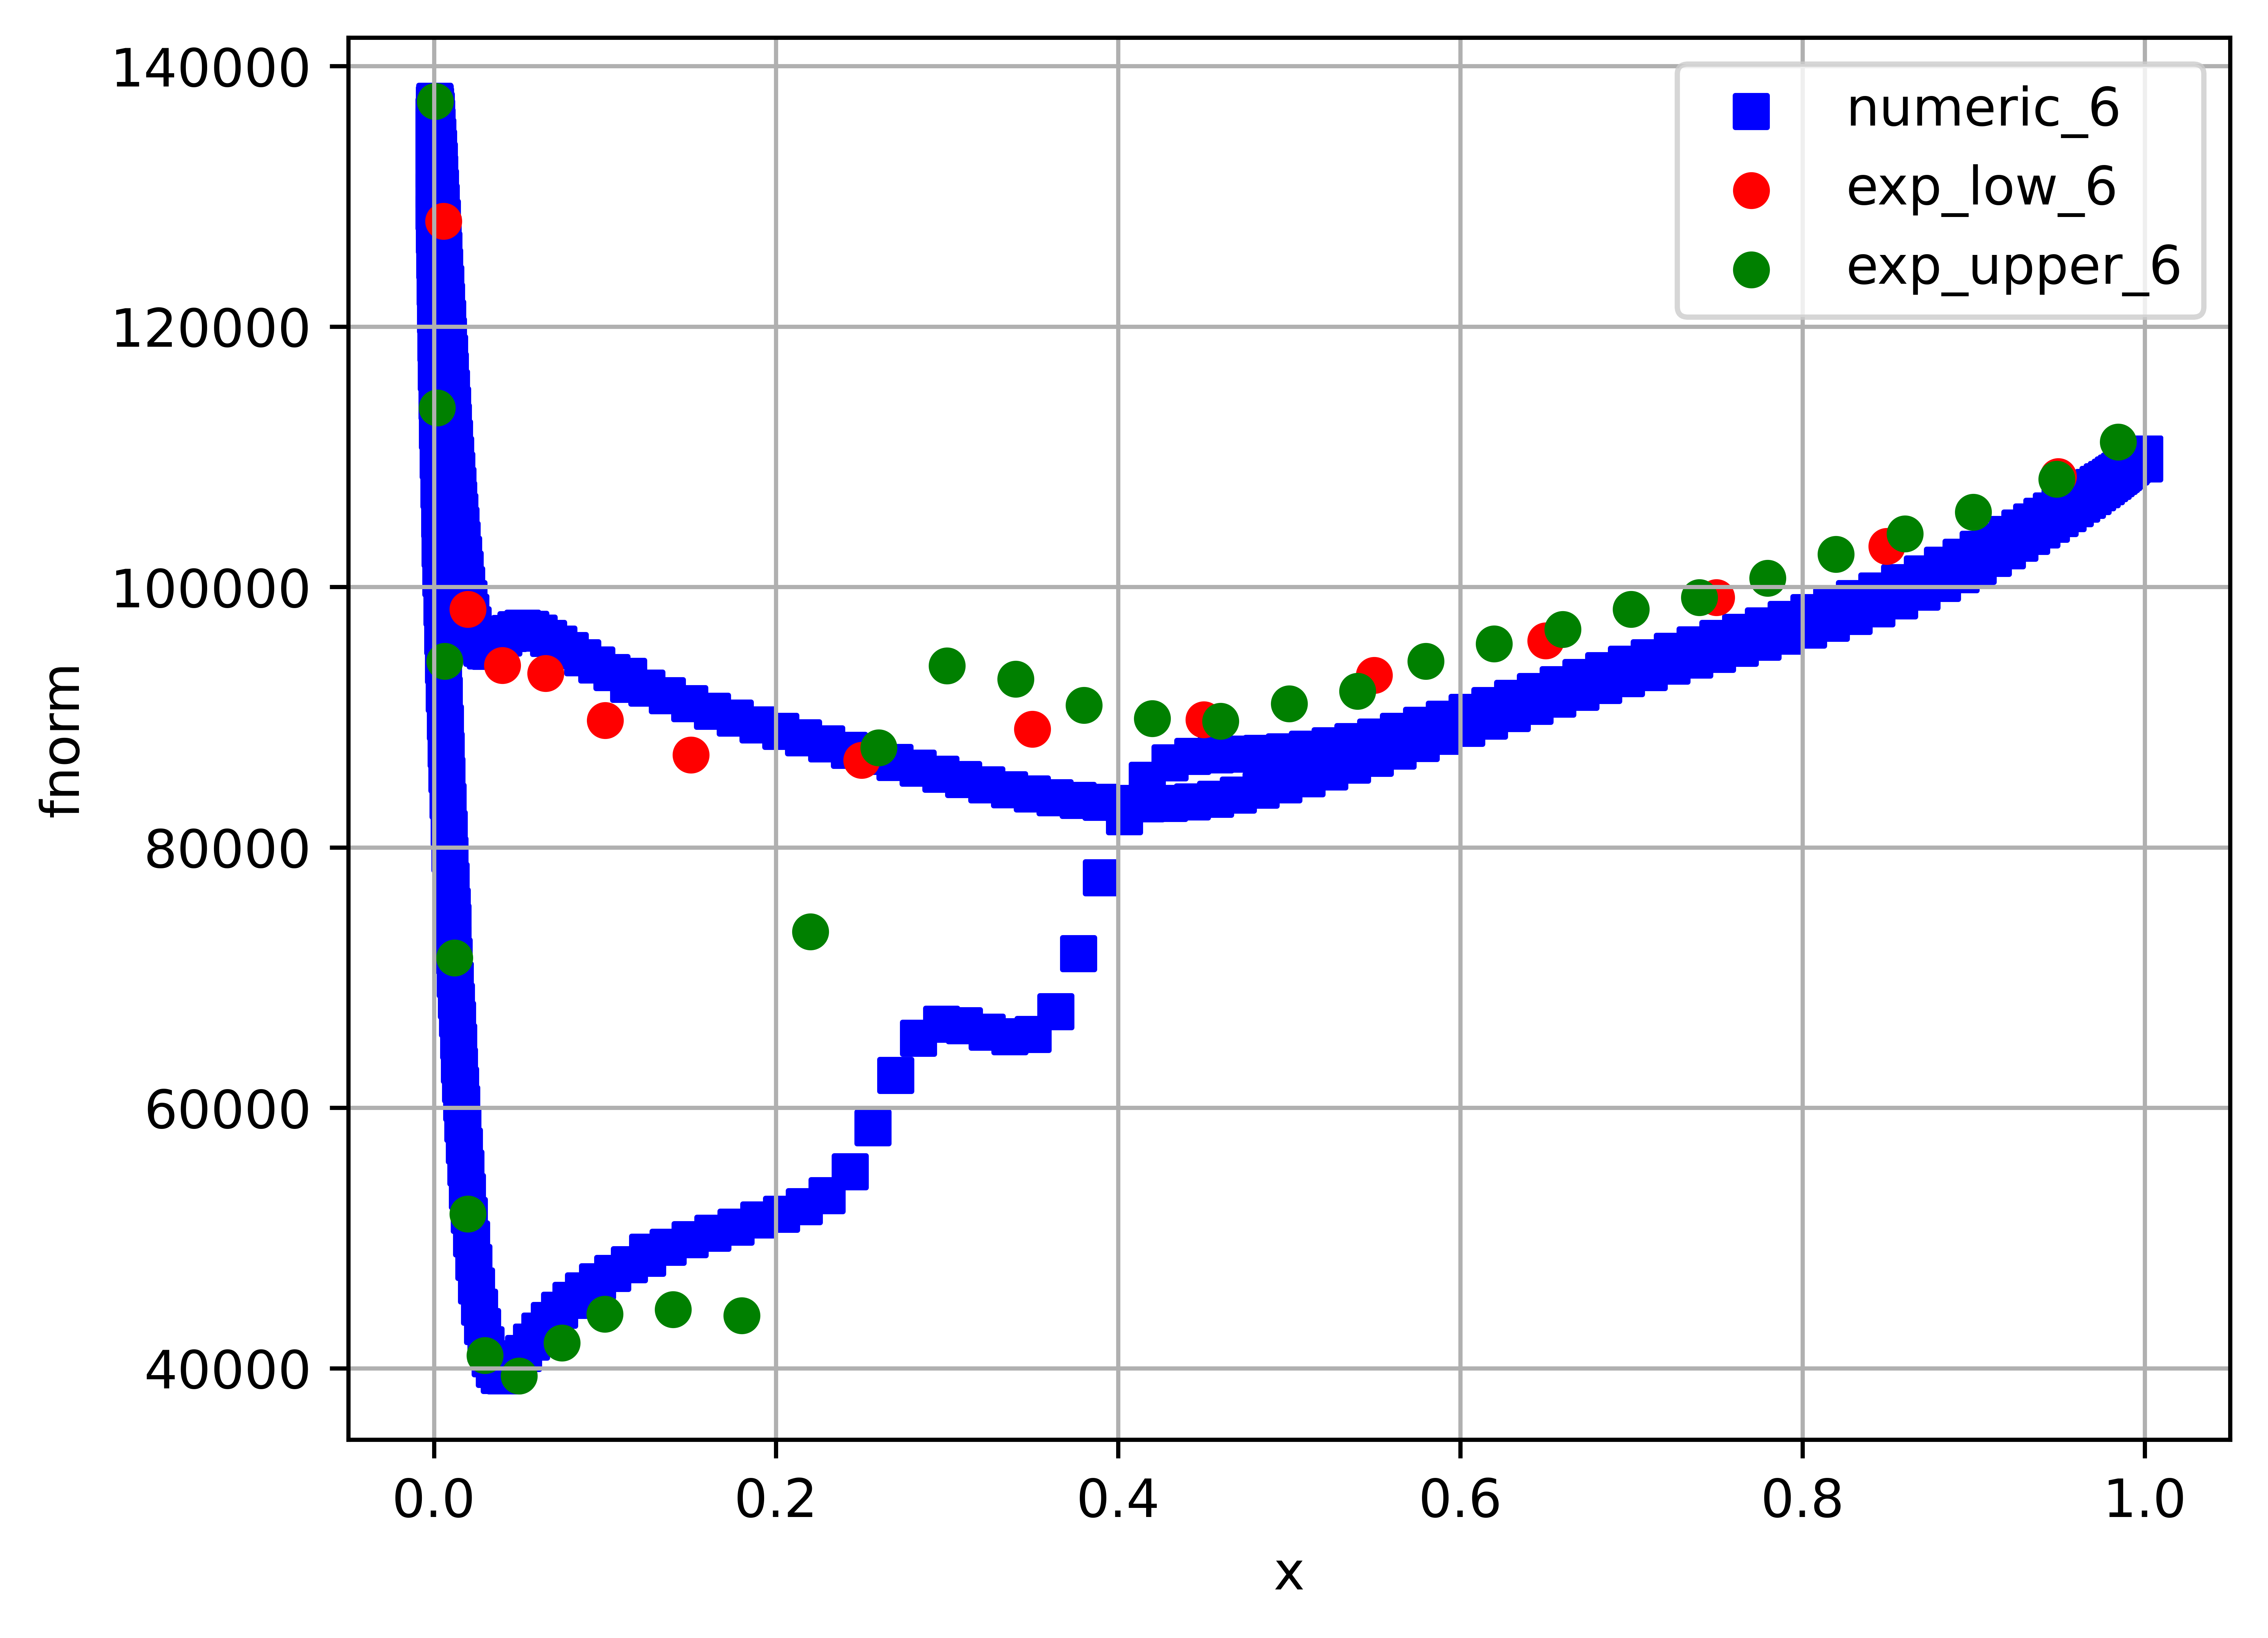
\includegraphics[width = 1\textwidth]{6.png}
\end{minipage}
\begin{minipage}{.49\textwidth}
    \centering
    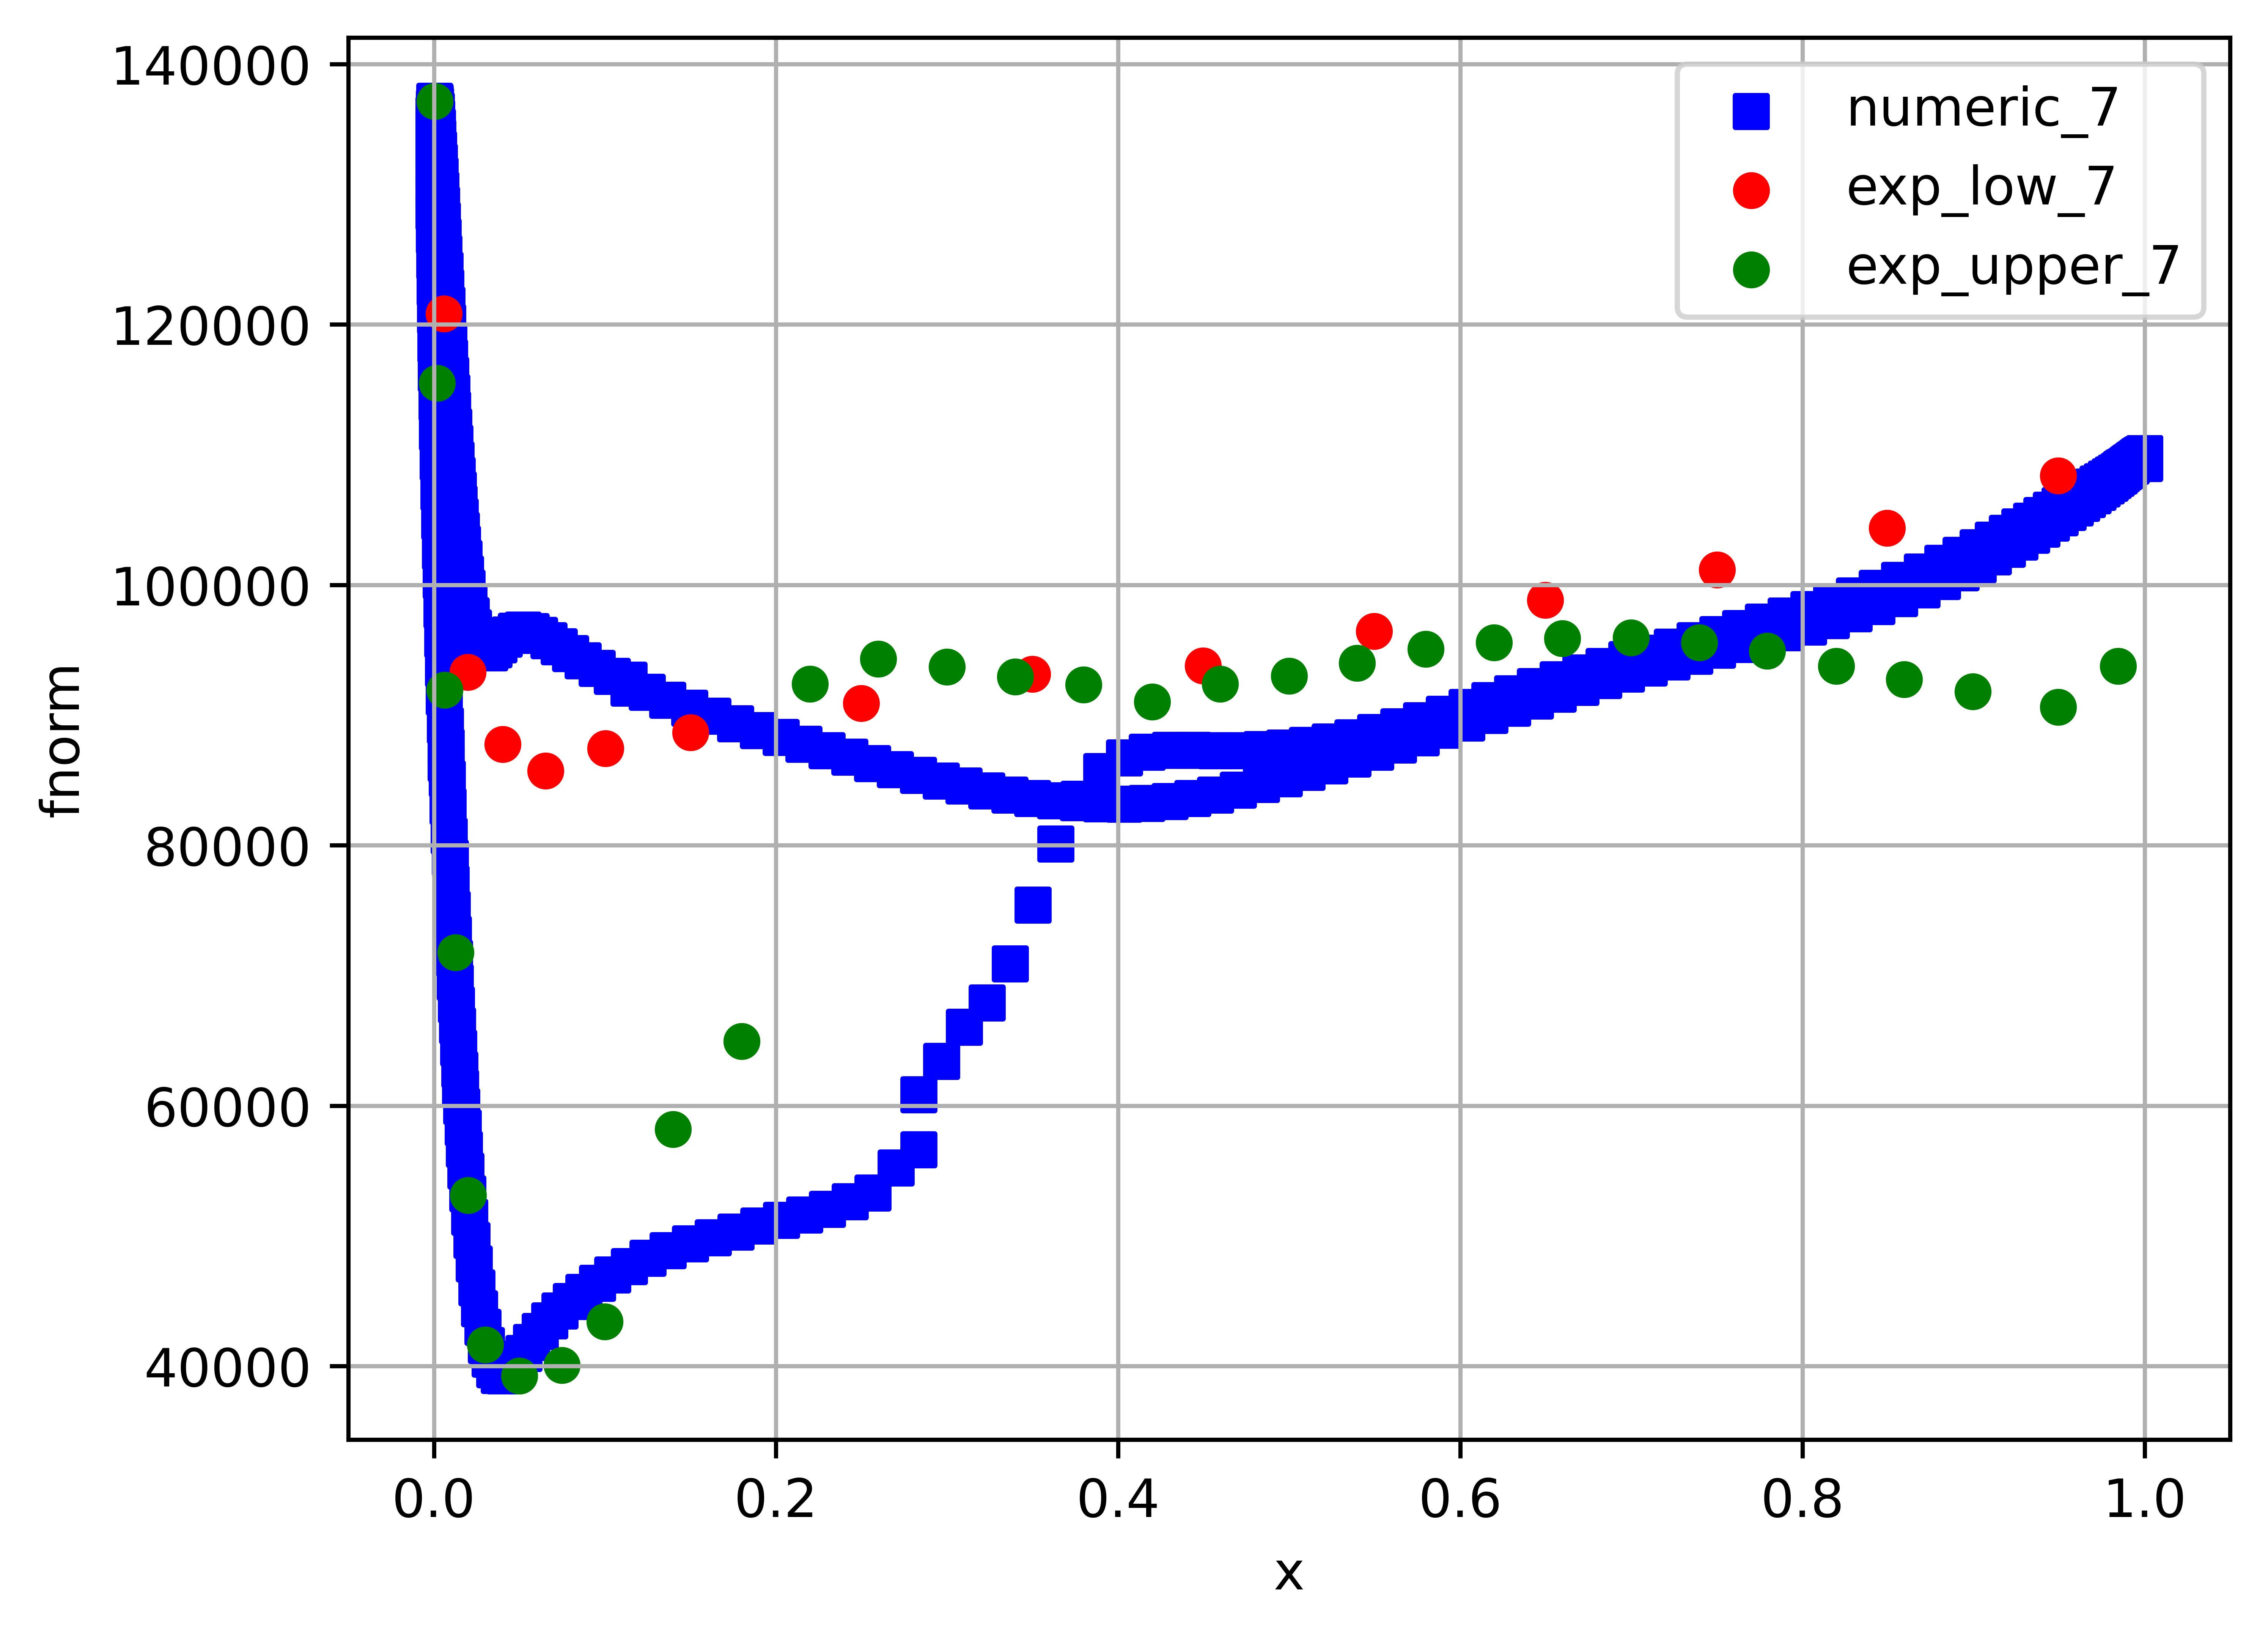
\includegraphics[width = 1\textwidth]{7.png}
\end{minipage}
\end{figure}
\end{document}